%\paragraph{Intro}
Psychoacoustics is the science of auditory perception and the human experience of hearing.
Limitations induced by the psychological and physiological mechanisms responsible for hearing are of particular 
interest and have been successfully applied to musical composition, architecture, digital audio coding, and mixing/rendering 
sound.
%and in particular the limitations induced by the psychological and physiological
%mechanisms responsible for the experience of hearing.
Individual psychoacoustic effects and illusions are refered to as \emph{psychoacoustic principles} and include:

\begin{itemize}
\item The Absolute Threshold of Hearing
\item Critical Band Frequency Analysis
\item Simultaneous Masking
\item Non-Simultaneous Masking
\item The Spread of Masking
\end{itemize}

In this method we seek to demonstrate how these basic psychoacoustic principles can be leveraged in a geometric sound propagation 
pipeline, with our most novel contribution being the use of masking in the propagation phase of sound simulation.

\paragraph{Auditory Filters and the Bark Scale of Critical Bandwidths}
%The frequency of sound is conventionally measured in hertz but alternative scales based on human perception are more commonly used
%in psychoacoustic literature and models.
%These include the Bark and ERB frequency scales, both of which are based on the frequency resolution of human hearing and are derived 
%from listening experiments.
%Although sound frequency is conventionally measured in hertz, for the purpose of psychoacoustic modelling it is preferable to use a 
%scale based on the frequency resolution of human hearing.
%The most common scale used in psychoacoustic literature is the Bark scale, which has units directly proportional to the frequency-dependent 
%bandwidth at which individual tones can be perceived separately.
%The Bark scale is measured in \textbf{critical bands}, 
%Frequency scales based on the resolution of human hearing are used for modelling psychoacoustic principles, most commonly the Bark scale.
%The Bark scale is measured in units of \emph{critical bands}

The perception of sound frequency is mediated by the \textbf{basilar membrane}, a coiled structure of the inner ear that vibrates in response 
to sound energy.
Regions of the basilar membrane have a characteristic frequency they are most sensitive to. This characteristic frequency is highest at the 
base of the basilar membrane and continuously decreases along it's length.
\paragraph{}
Pure tones result in patterns of excitation on the basilar membrane that may overlap for sounds that are nearby in frequency, and for this reason the 
basilar membrane is abstracted in literature as a bank of overlapping \textbf{auditory filters}.
%The bandwidth of an auditory filter is referred to as it's \textbf{critical bandwidth}
\textbf{The Bark frequency scale} is measured in units of the frequency-dependent bandwidths of the auditory filters of the basilar membrane, refered 
to as the \textbf{critical bandwidths}, and is a commonly used frequency scale in psychoacoustics because it is directly proportional to the frequency 
resolution of human hearing.
%whose bandwidths are measured by \textbf{the Bark scale}.
%Both the Bark scale and the curves representing auditory filters along the basilar membrane have been derived from listening experiments.
%The shape of these auditory filters have been derived from listening experiments and used to design a frequency scale proportional to the 
%frequency resolution of human hearing
%, and this overlap 
%has been measured through listening experiments.
\paragraph{Spectral Masking}
\begin{figure}
  \centerline{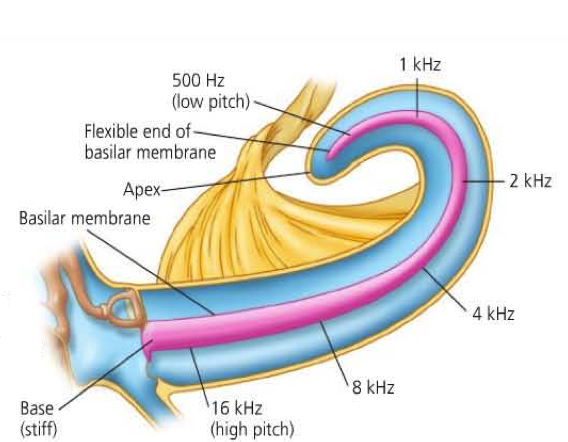
\includegraphics[width=2.8in]{figs/bmem}}
  \caption{The basilar membrane}
  \label{fig:basilarmembrane}
\end{figure}

\begin{figure}
  \centerline{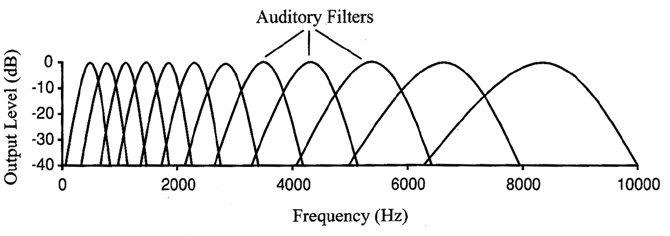
\includegraphics[width=2.8in]{figs/auditoryfilters}}
  \caption{Curves representing the response of auditory filters as a function of center frequency}
  \label{fig:auditoryfilters}
\end{figure}
Because of the observed overlap of auditory filters, a loud tone will also excite regions of the basilar membrane
that should correspond to neighboring frequencies. 
This interference of excitation is the phenomenon of \textbf{spectral masking}, where a tone played at a given 
frequency will perceptually occlude relatively softer tones that are nearby in frequency.
The intensity of masking is assymetric in frequency with lower tones masking higher tones with a higher intensity
than the reverse.
This psychoacoustic principle has been referred to as \textbf{the upward spread of masking} (the axis of `upward' being frequency).
\paragraph{}
\begin{figure}
  \centerline{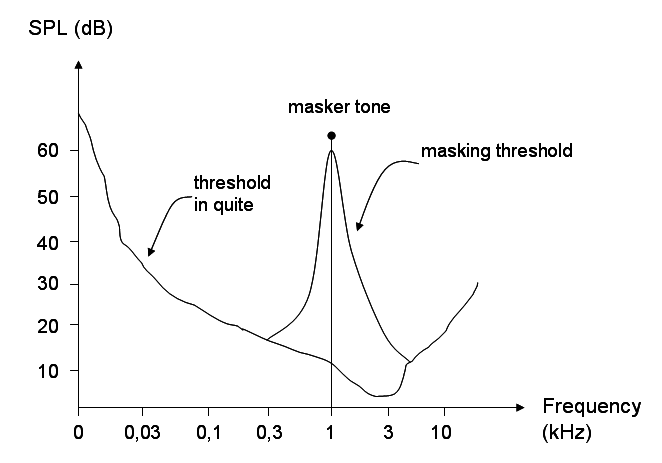
\includegraphics[width=2.8in]{figs/masked}}
  \caption{Absolute threshold of hearing and masked threshold}
  \label{fig:masked}
\end{figure}
The \textbf{absolute threshold of hearing} is a curve of minimum pressure level necessary to perceive a sound at 
a given frequency and in the presence of relative quiet.
Similarly, a \textbf{masking threshold} characterizes the threshold below which a sound is made imperceptible
in the presence of a masker.
The net result of spectral masking in the presence of multiple tones is approximately additive, and the net amount of 
masking continues to effect later tones after the masking tone has ended because of a phenomenon referred to as \textbf{non-simultaneous} or \textbf{temporal masking}.

%The basilar membrane is the auditory equivalent of the human eyes.
%It mediates human auditory perception as well as the phenomenon of spectral masking.
%The following is a brief overview of it's function as it relates to psychoacoustic principles.
